
\documentclass[acmtog]{acmart}

\usepackage{graphicx}
\usepackage{subcaption}
\usepackage{hyperref}

\graphicspath{ {./images/} }

\AtBeginDocument{%
	\providecommand\BibTeX{{%
			\normalfont B\kern-0.5em{\scshape i\kern-0.25em b}\kern-0.8em\TeX}}}

\setcopyright{acmcopyright}
\copyrightyear{2023}
\acmYear{2023}
\acmDOI{XXXXXXX.XXXXXXX}

\begin{document}
	\title{Land Use Classification Project Proposal}
	
	\author{Thai La}
	\email{vtl932@usask.ca}
	\orcid{1234-5678-9012}
	\affiliation{%
		\institution{University of Saskatchewan}
		\streetaddress{105 Administration Pl}
		\city{Saskatoon}
		\state{Saskatchewan}
		\country{Canada}
		\postcode{S7N 5A2}
	}
	
	\keywords{Satellite, Image, Classification, LandUse, GeoSpatial}
	
	\maketitle
	
	\section{Introduction}
	This report will outline the structure and approach used to solve the satellite land use image classification problem.\\
	\href{https://git.cs.usask.ca/vtl932/cmpt318_course_project}{The project repository can be found here}.\\
	\href{https://www.kaggle.com/datasets/apollo2506/eurosat-dataset?select=EuroSAT}{The Kaggle Dataset can be found here}.
	
	\section{Pre-processing}
	The data set of satellite images provided by Kaggle is well prepared. All provided images are 64x64 RGB images and has a Ground Sampling size of 10 meters. The images do not appear to contain any significant noise that warrants de-noising to occur. Furthermore, all JPG and csv files are not corrupted. However, the provided TIF files do not work; I was not able to open these TIF files in any sort of application. The TIF files are in EuroSatData/allBands.\\
	Typically, the RGB values for images are between (0,255), however, I will be working with the range (0,1) for these images; in other words, I will be working with the images in float instead of unsigned integers.
	
		\subsection{Data set split}
		
		The training, validation, and test split for the image data set is already provided along side the images. The splits are detailed in the train.csv, validation.csv and test.csv files. The given splits contain 70\% for  training, 20\% for validation and 10\% for testing. I will be using the given data set splits to train the model.
	
	\section{Approach}
	
	For classifying the images in the data set, a Convolutional Neural Network will be used to extract and learn good features, then a regular Artificial Neural Network will be used for classifying the image. The Convolutional Neural Network's learned features will be fed as input into the Artificial Neural Network to be used for classifying the image. Since it is a multi-classification problem, the Artificial Neural Network will be using SoftMax at the output layer to predict which class the image belongs to.\\
	From researching possible architectures, the VGG16 architecture seems the most promising for image classifications. As a result, I will implementing a model using the VGG16 model and tuning it to my use case, which is land use classification. I will first freeze the CNN layers and fine tune the dense layers to fit my use case. Then adjust any hyper-parameters as needed when training and validating.\\
	I will also train another model by manually setting up the layers of the model. The results from the two models will be compared and the best performing model will be selected as the final model for submission.\\
	For implementing these neural network models in code, I will be using the tensorflow library in Python. 
	Some important parameters used to fit the model will include:
	\begin{itemize}
		\item epoch: specify how many iterations the model will be trained for
		\item batch\_size: specify the batch size for training
		\item training\_data: the data set used for training, including the x and y data set.
		\item learning\_rate: the pace at which the algorithm updates its weights
		\item schedule: a schedule to specify the decay or decrease of the learning rate
	\end{itemize}
	
	In terms of tensorflow implementation, convolution layers will be used to learn good features, then they are flattened and inputted into a regular dense layer for prediction.
	
	
	\section{Measures of Performance}
	
	Some metrics used to gauge performance of the models will be the accuracy metric, the loss metric, the recall metric, and the precision metric. Naturally, the recall and precision metric will be produced from a confusion matrix, which will be included as a table/matrix as part of the performance report.\\
	The confusion matrix, recall metric and precision metric are new additions to my Proposed Results which were not present in the previously submitted Project Proposal.


	\begin{figure*}[h]
		\centering
		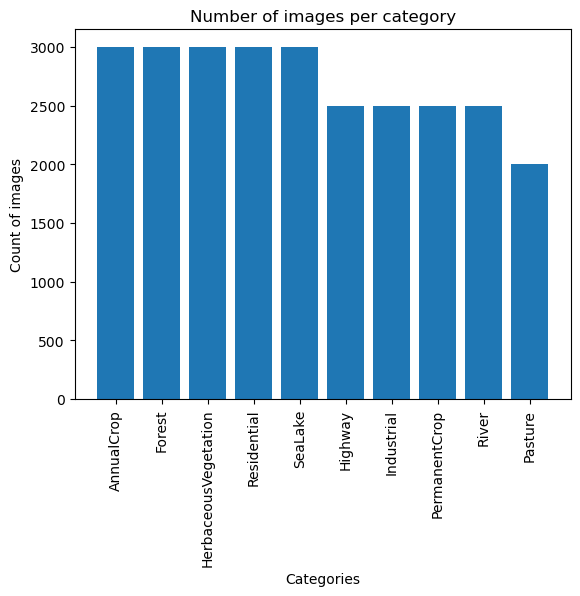
\includegraphics[scale=0.7]{src/images/Fig1.png}\\
		Figure 1. Dataset Figure - Number of images per category label
		
		\vspace{2cm}
		
		\centering
		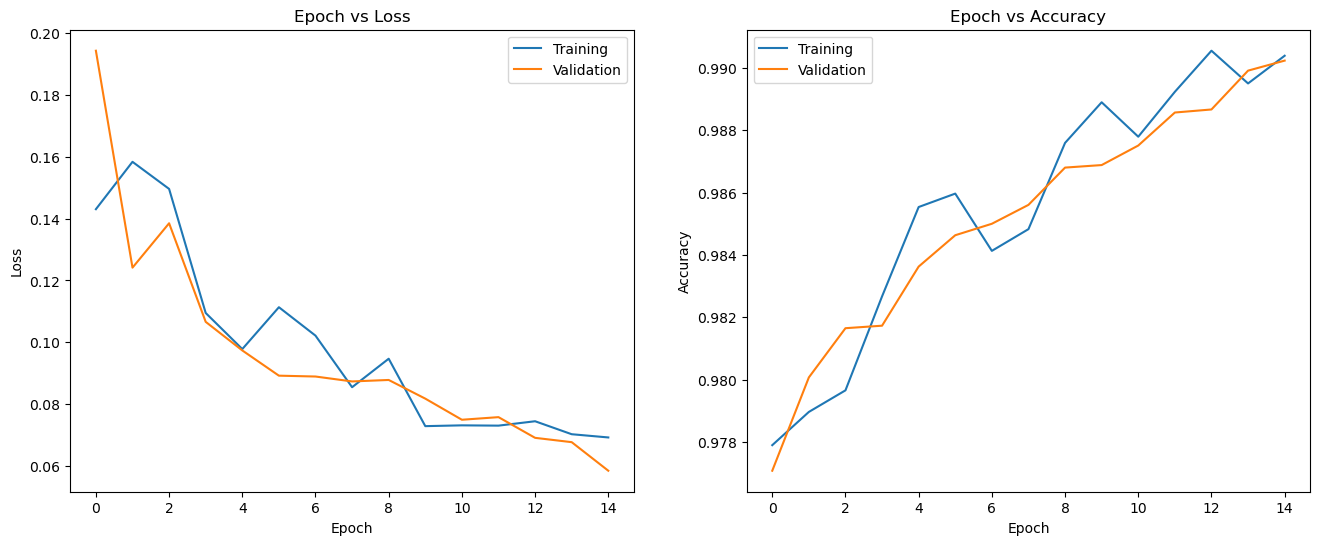
\includegraphics[scale=0.5]{src/images/Fig3.png}\\
		Figure 2a. Proposed Results figure - Accuracy and Loss measured at each Epoch
	\end{figure*}
	
	
	\begin{figure*}[h]
		\centering
		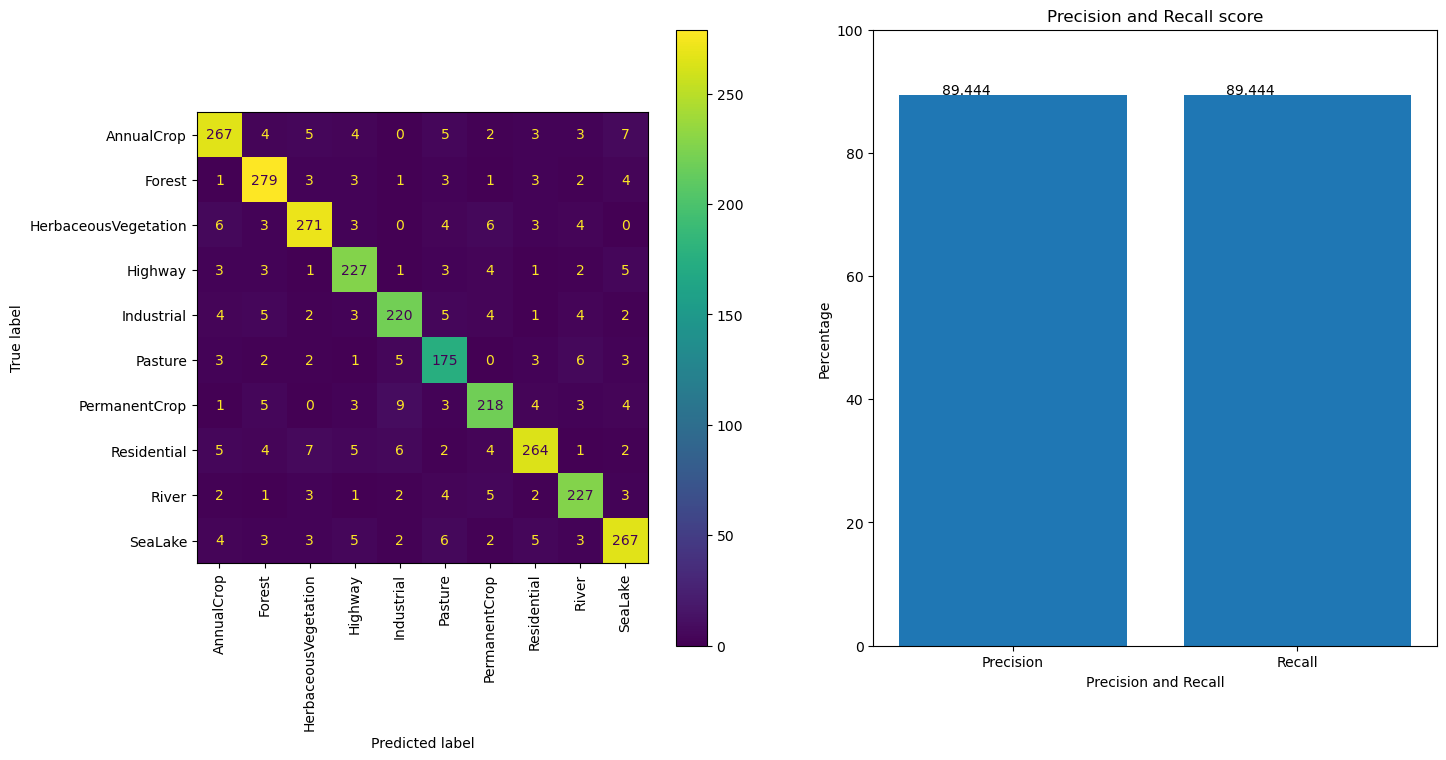
\includegraphics[scale=0.5]{src/images/Fig3b.png}\\
		Figure 2b. Proposed Results figure - Confusion Matrix and its corresponding Recall and Precision scores
	\end{figure*}
\end{document}
\endinput
